\documentclass[tikz,border=5mm,12pt]{standalone}
\usetikzlibrary{positioning,shapes.geometric}

\begin{document}
  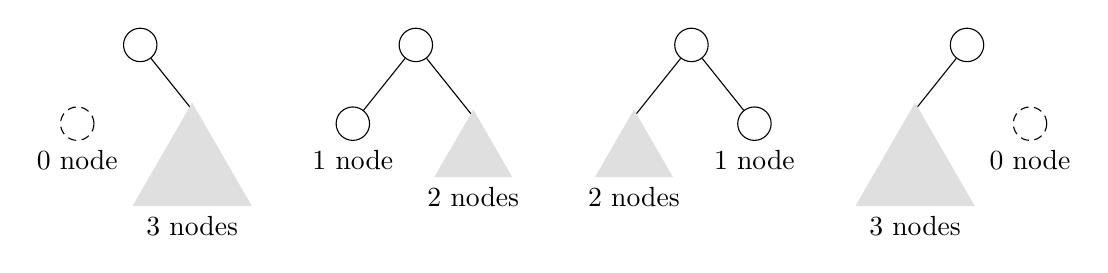
\begin{tikzpicture}[
    treenode/.style={
      circle,draw,inner sep=1.5mm
    },
    emptynode/.style={
      treenode,
      densely dashed
    },
    tree/.style={
      level distance=10mm,
      level 1/.style={sibling distance=16mm,align=center},
      every node/.style={
        anchor=center
      }
    },
    subtree/.style={
      fill=lightgray!50,
      isosceles triangle,
      isosceles triangle apex angle=60,
      shape border rotate=90
    }]

      \begin{scope}[tree]
        \node[treenode] {}
          child {node[emptynode,label=below:{0 node}] {} edge from parent[draw=none]}
          child {node {}
            {node[subtree,label=below:{3 nodes},xshift=-4pt,yshift=-14pt] {\huge$\strut$}}
          };
      \end{scope}

      \begin{scope}[tree,xshift=35mm]
        \node[treenode] {}
          child {node[treenode,label=below:{1 node}] {}}
          child {node {}
            {node[subtree,label=below:{2 nodes},xshift=-2pt,yshift=-10pt] {$\strut$}}
          };
      \end{scope}

      \begin{scope}[tree,xshift=70mm]
        \node[treenode] {}
          child {node {}
            {node[subtree,label=below:{2 nodes},xshift=2pt,yshift=-10pt] {$\strut$}}
          }
          child {node[treenode,label=below:{1 node}] {}};
      \end{scope}

      \begin{scope}[tree,xshift=105mm]
        \node[treenode] {}
          child {node {}
            {node[subtree,label=below:{3 nodes},xshift=4pt,yshift=-14pt] {\huge$\strut$}}
          }
          child {node[emptynode,label=below:{0 node}] {} edge from parent[draw=none]};
      \end{scope}
  \end{tikzpicture}
\end{document}
